\documentclass[twocolumn,10pt]{aastex631}

% ---------- Packages ----------
\usepackage{amsmath,amssymb}
\DeclareMathOperator*{\argmin}{arg\,min}
\DeclareMathOperator*{\argmax}{arg\,max}
\usepackage{graphicx}
\usepackage{booktabs}
\usepackage{multirow}
\usepackage{float}

\usepackage{tikz}
\usetikzlibrary{arrows.meta,positioning,fit,calc,backgrounds}

\shorttitle{BCG Candidate Classification with Uncertainty Quantification}
\shortauthors{Machine Learning Documentation}

\begin{document}

\title{Machine Learning Architecture for Brightest Cluster Galaxy Candidate Classification: A Probabilistic Approach with DES Prior Integration}

\author{Documentation of Implementation}
\affiliation{High Energy Physics Image Marker Project}

\begin{abstract}
We present a machine learning framework for identifying Brightest Cluster Galaxies (BCGs) that combines optical imaging data with auxiliary astronomical measurements through neural network architectures providing both deterministic classifications and probabilistic outputs. Our approach employs a two-stage pipeline: (1) candidate identification via either automatic local maxima detection or DES photometric prior catalogs, and (2) feature-based classification using multi-layer perceptrons with optional uncertainty quantification through Monte Carlo dropout and temperature scaling. The system processes BCG datasets at 2.2 and 3.8 arcminute scales, incorporating redshift and stellar mass indicators ($\Delta m^*_z$) as additional features. We implement supervised training using RedMapper BCG probabilities for loss weighting while excluding these probabilities from inference features to prevent data leakage. This framework addresses key challenges in automated BCG identification by providing calibrated confidence estimates essential for large-scale astronomical surveys.
\end{abstract}

\keywords{methods: data analysis --- galaxies: clusters: general --- techniques: image processing --- methods: statistical}

\section{Introduction}

The identification of Brightest Cluster Galaxies (BCGs) represents a fundamental challenge in extragalactic astronomy, requiring integration of photometric, morphological, and contextual information. Traditional approaches relying on manual inspection or simple brightness-based selection become computationally prohibitive for modern large-scale surveys such as the Dark Energy Survey (DES) \citep{Rykoff2016}.

\subsection{Historical Context of Feature Extraction in Astronomical Machine Learning}

The evolution of feature extraction methods in astronomy has undergone significant transformation over the past two decades. Early quantitative approaches to galaxy morphology relied heavily on handcrafted features, most notably the CAS system (Concentration, Asymmetry, Smoothness) introduced by \citet{Abraham1996} and later extended by \citet{Conselice2003}. These parametric measures provided objective quantification of galaxy structure, enabling systematic morphological classification across large datasets such as the Sloan Digital Sky Survey (SDSS).

The CAS parameters represent the foundational paradigm of engineered feature extraction in astronomical applications. Concentration measures the central light distribution, asymmetry quantifies rotational symmetry deviations, and smoothness captures small-scale structural irregularities \citep{Conselice2003}. Extensions to this system included Gini coefficients and $M_{20}$ moments \citep{Hambleton2011}, creating comprehensive morphometric frameworks that enabled robust statistical analysis of galaxy populations.

Traditional feature engineering approaches demonstrated remarkable success in characterizing galaxy morphologies and enabled discoveries about galaxy evolution across cosmic time \citep{Conselice2014}. However, these methods required extensive domain expertise to design appropriate features and often failed to capture subtle morphological variations that might be astronomically significant.

The paradigm shifted dramatically with the advent of deep learning approaches in the 2010s, where convolutional neural networks (CNNs) began extracting features automatically through hierarchical representation learning \citep{Dieleman2015}. This transition from handcrafted to learned features marked a fundamental change in astronomical data analysis, enabling detection of patterns beyond human-engineered parametrizations.

\subsection{Contemporary Challenges and Hybrid Approaches}

Recent work in BCG detection reflects this methodological evolution. \citet{Janulewicz2025BCG} demonstrated that neural networks can achieve 95\% accuracy in automated BCG identification using purely data-driven approaches, while \citet{COSMIC2024} developed the COSMIC algorithm combining traditional clustering methods with machine learning techniques for improved cluster detection.

However, purely data-driven approaches face significant challenges in astronomical contexts. Deep learning models often lack interpretability crucial for scientific validation, require extensive training data that may not be available for rare astronomical objects, and can struggle with domain adaptation across different surveys or instruments. Furthermore, the physical understanding embedded in traditional parametric features remains valuable for incorporating known astrophysical relationships.

\subsection{The Case for Hybrid Feature Integration}

Our approach addresses these limitations by implementing a hybrid framework that combines the interpretability and physical grounding of engineered features with the flexibility of modern machine learning architectures. This methodology enables incorporation of auxiliary astronomical measurements (redshift, stellar mass indicators) that provide crucial physical context unavailable to purely image-based approaches.

The integration of uncertainty quantification through Monte Carlo dropout \citep{Laves2019WellCalibratedMU} and temperature scaling addresses a critical gap in astronomical machine learning applications, where quantified confidence estimates are essential for scientific decision-making and pipeline integration in large-scale surveys.

We present a machine learning framework that reformulates BCG identification as a candidate classification problem, providing both deterministic rankings and probabilistic outputs with uncertainty quantification. Our approach naturally handles the discrete nature of galaxy identification while incorporating diverse astronomical data products, bridging traditional parametric methods with modern probabilistic inference techniques.

\section{System Architecture}

Figure~\ref{fig:architecture} presents the complete machine learning pipeline, illustrating data flow from optical inputs through candidate selection, feature extraction, neural network processing, and probabilistic inference.

% =========================================================
% Figure: Two-row layout matching actual Python implementation
% =========================================================


\begin{figure*}[t]
\centering
\resizebox{\textwidth}{!}{
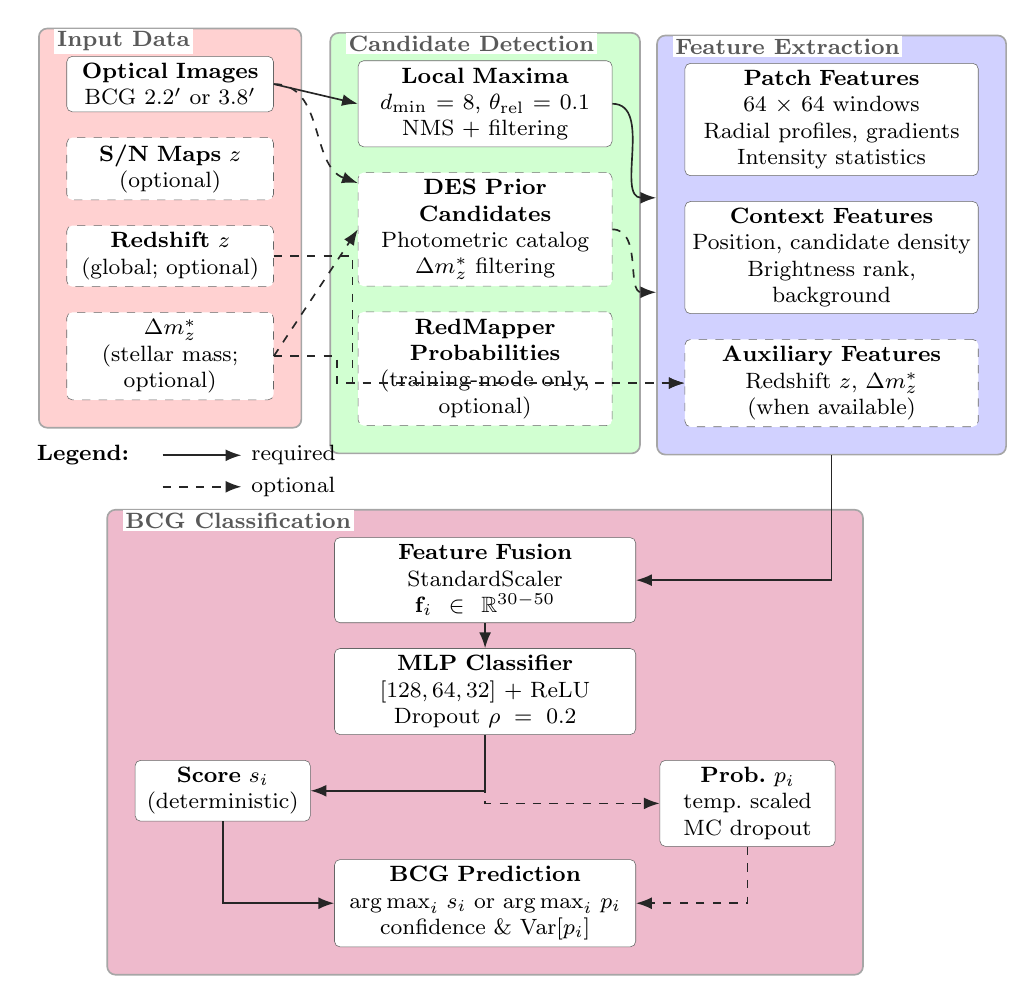
\begin{tikzpicture}[
  font=\footnotesize,
  node distance=6mm and 9mm,
  >=Latex,
  every node/.style={align=center},
  box/.style={rounded corners=2pt, draw=black!60, very thin, fill=white, inner sep=2.5pt},
  data/.style={box},
  optdata/.style={box, dashed},         % optional data boxes (dashed border)
  proc/.style={box},
  feat/.style={box},
  optfeat/.style={box, dashed},         % optional feature boxes (dashed border)
  nn/.style={box},
  outbox/.style={box},                  % avoid TikZ 'out' key name
  reqedge/.style={-Latex, semithick, draw=black!85},
  optedge/.style={-Latex, semithick, dashed, draw=black!85},
  panel/.style={rounded corners=3pt, draw=black!35, line width=0.6pt, inner sep=3.5mm, fill opacity=0.90},
  ptitle/.style={font=\bfseries\footnotesize, text=black!65, fill=white, inner sep=1pt}
]
\def\vsep{3.2mm} % uniform vertical gap

% -------------------- FIRST ROW: Inputs, Detection, Features --------------------
% Columns: Inputs (x=0), Detection (x=4.0), Features (x=8.4)

% INPUTS
\begin{scope}[xshift=0cm, yshift=0cm]
  \node[data,    text width=2.45cm] (Opt) at (0, 1.50) {\textbf{Optical Images}\\BCG 2.2$'$ or 3.8$'$};
  \node[optdata, text width=2.45cm] (SN)   [below=\vsep of Opt] {\textbf{S/N Maps $z$}\\(optional)};
  \node[optdata, text width=2.45cm] (Z)   [below=\vsep of SN] {\textbf{Redshift $z$}\\(global; optional)};
  \node[optdata, text width=2.45cm] (Delta)   [below=\vsep of Z] {\textbf{$\Delta m^*_z$}\\(stellar mass; optional)};
\end{scope}

% CANDIDATE DETECTION
\begin{scope}[xshift=4.0cm, yshift=0cm]
  \node[proc, text width=3.05cm] (Det) at (0, 1.25)
    {\textbf{Local Maxima}\\$d_{\min}=8$, $\theta_{\mathrm{rel}}=0.1$\\NMS + filtering};
  \node[proc, text width=3.05cm, dashed, draw=black!55] (DES) [below=\vsep of Det]
    {\textbf{DES Prior Candidates}\\Photometric catalog\\$\Delta m^*_z$ filtering};
  \node[proc, dashed, text width=3.05cm] (RedM) [below=\vsep of DES]
    {\textbf{RedMapper \\ Probabilities}\\(training-mode only, \\optional)};

  % Input connections to detection (clean routes)
  \path[reqedge] (Opt.east) -- (Det.west);
  \path[optedge] (Opt.east) to[out=0,in=160] (DES.160);
  \path[optedge] (Delta.east) -- (DES.west);
\end{scope}

% FEATURE EXTRACTION (slightly lowered; includes patch-based features)
\begin{scope}[xshift=8.4cm, yshift=-9mm]
  \node[feat, text width=3.55cm] (Patch)  at (0, 1.95) {\textbf{Patch Features}\\$64 \times 64$ windows\\Radial profiles, gradients\\Intensity statistics};
  \node[feat,    text width=3.55cm] (Context) [below=\vsep of Patch]  {\textbf{Context Features}\\Position, candidate density\\Brightness rank, background};
  \node[optfeat,    text width=3.55cm] (Aux) [below=\vsep of Context] {\textbf{Auxiliary Features}\\Redshift $z$, $\Delta m^*_z$\\(when available)};
\end{scope}

% -------------------- SECOND ROW: Fusion & Classification (fully below row-1) --------------------
\begin{scope}[xshift=40mm, yshift=-70mm]  % set well below row-1 to avoid overlap
  % Fusion
  \node[nn, text width=3.65cm] (Fusion) at (0, 2.2)
    {\textbf{Feature Fusion}\\StandardScaler\\$\mathbf{f}_i \in \mathbb{R}^{30-50}$};

  % Classifier with correct architecture
  \node[nn, text width=3.65cm] (CLS) [below=\vsep of Fusion]
    {\textbf{MLP Classifier}\\$[128, 64, 32]$ + ReLU\\Dropout $\rho = 0.2$};

  % Outputs (deterministic and probabilistic)
  \node[outbox, text width=2.05cm] (Score) [below left=\vsep and 3mm of CLS] {\textbf{Score $s_i$}\\(deterministic)};
  \node[outbox, text width=2.05cm] (Prob)  [below right=\vsep and 3mm of CLS] {\textbf{Prob.\ $p_i$}\\temp.\ scaled\\MC dropout};

  % Decision centered below
  \node[outbox, text width=3.65cm] (Dec) [below=\vsep of $(Score.south)!0.5!(Prob.south)$]
    {\textbf{BCG Prediction}\\$\argmax_i\,s_i$ or $\argmax_i\,p_i$\\confidence \& $\mathrm{Var}[p_i]$};

  % Inside-panel flow
  \path[reqedge] (Fusion) -- (CLS);
  \path[reqedge] (CLS.south) |- (Score.east);
  \path[optedge] (CLS.south) |- (Prob.west);
  \path[reqedge] (Score.south) |- (Dec.west);
  \path[optedge] (Prob.south) |- (Dec.east);

  % Background panel and title (inside)
  \begin{pgfonlayer}{background}
    \node[panel, fill=purple!30, fit=(Fusion)(CLS)(Score)(Prob)(Dec)] (PFuse) {};
  \end{pgfonlayer}
  \node[ptitle, anchor=west] at ($(PFuse.north west)+(2mm,-1.5mm)$) {BCG Classification};
\end{scope}

% ==================== STAGE PANELS (ROW-1) & TITLES ====================
\begin{pgfonlayer}{background}
  \node[panel, fill=red!20,  fit=(Opt)(Z)(Delta)]                              (PIn)   {};
  \node[panel, fill=green!20, fit=(Det)(DES)(RedM)]                              (PDet)  {};
  \node[panel, fill=blue!20,fit=(Patch)(Context)(Aux)]            (PFeat) {};
\end{pgfonlayer}
\node[ptitle, anchor=west] at ($(PIn.north west)+(2mm,-1.7mm)$)   {Input Data};
\node[ptitle, anchor=west] at ($(PDet.north west)+(2mm,-1.5mm)$)  {Candidate Detection};
\node[ptitle, anchor=west] at ($(PFeat.north west)+(2mm,-1.5mm)$) {Feature Extraction};

% ===== Connections between Detection -> Feature Extraction (to panel edge, non-overlapping) =====
\path[reqedge] (Det.east)  to[out=0,in=180] ($(PFeat.west)+(0,6mm)$);
\path[optedge] (DES.east)   to[out=0,in=180] ($(PFeat.west)+(-0.0,-6mm)$);

% ===== Optional auxiliary features -> Feature Extraction (long dashed, elbow; avoids labels) =====
\coordinate (Zmid) at ($(Z.east)+(1.0,0)$);
\path[optedge] (Z.east) -- (Zmid) |- (Aux.west);
\coordinate (Deltamid) at ($(Delta.east)+(0.8,0)$);
\path[optedge] (Delta.east) -- (Deltamid) |- (Aux.west);

% ===== Single arrow from bottom of Feature Extraction panel -> Feature Fusion =====
\path[reqedge] (PFeat.south) |- (Fusion.east);

% ==================== LEGEND ====================
\node[draw=none, anchor=west] (LegTitle) at ($(Delta.south west)+(-5mm,-7mm)$) {\textbf{Legend:}};
\draw[reqedge] (LegTitle.east) ++(3mm,0) -- ++(10mm,0) node[right, black] {\footnotesize required};
\draw[optedge] (LegTitle.east) ++(3mm,-4mm) -- ++(10mm,0) node[right, black] {\footnotesize optional};

\end{tikzpicture}%
} % end resizebox


\caption{BCG candidate classification architecture. The system processes optical astronomical data from BCG datasets through candidate selection (automatic local maxima detection or DES photometric priors), comprehensive feature extraction, neural network classification with optional uncertainty quantification, and probabilistic inference. Solid arrows indicate required components; dashed arrows show optional enhancements available based on data configuration. The framework supports both 2.2' and 3.8' scale BCG datasets with optional auxiliary features (redshift, stellar mass indicators).}
\label{fig:architecture}
\end{figure*}



\section{Methodology}

\subsection{Problem Formulation}

Rather than treating BCG identification as coordinate regression, we formulate it as a candidate ranking and classification task. Given an optical image $\mathbf{I} \in \mathbb{R}^{H \times W \times C}$ and optional auxiliary measurements $\mathbf{a} \in \mathbb{R}^{D_a}$ (redshift, stellar mass indicators), our objective is to:

\begin{enumerate}
\item Identify candidate locations $\mathcal{C} = \{(x_i, y_i)\}_{i=1}^{N}$ via automatic detection or prior catalogs
\item Extract feature representations $\mathbf{f}_i \in \mathbb{R}^{D}$ for each candidate
\item Classify each candidate with score $s_i$ (deterministic) or probability $p_i = P(\text{BCG}|\mathbf{f}_i)$ (probabilistic)
\item Select the highest-scoring candidate as the BCG prediction
\end{enumerate}

This formulation enables direct uncertainty quantification, natural handling of ambiguous cases, and principled integration of diverse observational constraints.

\subsection{Data Integration}

Our framework processes optical imaging data from BCG datasets at two angular scales:

\subsubsection{BCG Datasets}
The system supports BCG images at two scales:
\begin{itemize}
\item \textbf{2.2 arcminute scale}: Higher resolution images suitable for nearby clusters
\item \textbf{3.8 arcminute scale}: Wider field images accommodating more distant systems
\end{itemize}

Images are stored as multi-frame TIFF files with embedded WCS (World Coordinate System) information for astrometric calibration.

\subsubsection{Auxiliary Astronomical Measurements}
The system incorporates auxiliary measurements as global features:
\begin{itemize}
\item \textbf{Photometric Redshift}: $z$ provides distance and evolutionary context
\item \textbf{Stellar Mass Indicator}: $\Delta m^*_z$ represents magnitude difference from characteristic stellar mass, providing crucial constraints on galaxy properties
\end{itemize}

\subsection{Candidate Selection Strategies}

The framework supports two distinct candidate identification approaches:

\subsubsection{Automatic Candidate Detection}

The automatic detection system employs a multi-stage pipeline for identifying candidate BCG locations based on local intensity maxima, following established approaches in astronomical source detection \citep{Bertin1996}. This method adapts traditional peak-finding algorithms commonly used in photometric catalogs to the specific requirements of BCG identification within cluster environments.

\textbf{Preprocessing and Image Standardization}: The pipeline begins with image preprocessing to ensure consistent input format. Multi-band RGB images are converted to grayscale using standard luminance weighting:
\begin{equation}
L = 0.299 \cdot R + 0.587 \cdot G + 0.114 \cdot B
\end{equation}
This conversion preserves the primary luminosity information crucial for identifying the brightest objects while reducing computational complexity.

\textbf{Local Maxima Detection}: The core detection mechanism employs a 3×3 maximum filter implemented through \texttt{scipy.ndimage.maximum\_filter}, creating a binary mask where each pixel equals the maximum value in its local neighborhood. This approach identifies local intensity peaks while maintaining computational efficiency suitable for large-scale processing:
\begin{equation}
M(x,y) = \begin{cases} 
1 & \text{if } I(x,y) = \max_{(i,j) \in \mathcal{N}_3(x,y)} I(i,j) \\
0 & \text{otherwise}
\end{cases}
\end{equation}
where $\mathcal{N}_3(x,y)$ represents the 3×3 neighborhood centered at pixel $(x,y)$.

\textbf{Adaptive Intensity Thresholding}: To minimize spurious detections from noise and faint background sources, the system applies a relative intensity threshold $\theta_{\text{rel}} = 0.1$ (default) scaled by the image maximum:
\begin{equation}
T_{\text{abs}} = \theta_{\text{rel}} \cdot \max(\mathbf{I})
\end{equation}
Only local maxima exceeding this threshold are retained as candidate locations. This adaptive approach automatically adjusts to varying image dynamic ranges across different observations and survey depths.

\textbf{Border Exclusion}: Candidates within 30 pixels (default) of image boundaries are systematically removed to avoid edge artifacts and incomplete photometric measurements that could compromise feature extraction. This exclusion zone ensures sufficient context for subsequent patch-based feature computation.

\textbf{Non-Maximum Suppression (NMS)}: The final stage implements a greedy NMS algorithm to enforce spatial separation constraints and prevent multiple detections of the same astronomical object. Candidates are processed in descending brightness order, with each candidate retained only if it lies more than $d_{\min} = 8$ pixels from all previously selected candidates:
\begin{equation}
d_{ij} = \sqrt{(x_i - x_j)^2 + (y_i - y_j)^2} > d_{\min}
\end{equation}
This distance constraint reflects typical seeing conditions and prevents over-sampling of extended sources.

The algorithm terminates when either the desired number of candidates (\texttt{max\_candidates = 50}) is reached or all remaining maxima have been processed. This systematic approach ensures robust candidate identification while maintaining computational tractability for large datasets.

\subsubsection{DES Photometric Prior Candidates}

For datasets with existing photometric catalogs, our framework leverages pre-computed candidate selections from established astronomical pipelines, particularly the Dark Energy Survey (DES) photometric catalog and RedMapper cluster finder \citep{Rykoff2014redMaPPer,Rykoff2016}. This approach represents a paradigm shift from purely image-based detection to integration with existing astronomical knowledge products.

\textbf{RedMapper Integration and Red-Sequence Selection}: The RedMapper algorithm provides a sophisticated foundation for BCG candidate identification through its red-sequence cluster finding methodology \citep{Rykoff2014redMaPPer}. RedMapper identifies galaxy clusters by detecting overdensities of red-sequence galaxies at specific photometric redshifts, simultaneously providing estimates of cluster richness, photometric redshift, and preliminary BCG candidates. Our implementation utilizes RedMapper's BCG probability assignments during training supervision while carefully excluding these probabilities from inference features to prevent data leakage.

\textbf{Stellar Mass Filtering via $\Delta m^*_z$ Criteria}: A critical component of the DES prior approach involves filtering candidates based on the stellar mass indicator $\Delta m^*_z$, which represents the magnitude difference from the characteristic stellar mass at a given redshift \citep{Rykoff2016}. This parameter provides powerful constraints on galaxy selection by identifying objects with stellar masses consistent with BCG populations:
\begin{equation}
\Delta m^*_z = m_i - m^*(z)
\end{equation}
where $m_i$ is the observed magnitude of candidate $i$ and $m^*(z)$ is the characteristic magnitude corresponding to the break in the galaxy luminosity function at redshift $z$.

Candidates with $\Delta m^*_z$ values consistent with massive galaxy populations (typically $\Delta m^*_z < 1.0$) are preferentially retained, effectively pre-selecting objects with stellar masses appropriate for BCG identification. This filtering reduces the candidate pool size while maintaining high completeness for genuine BCGs.

\textbf{Computational Efficiency and Pipeline Integration}: The DES prior approach offers significant computational advantages over exhaustive image-based detection. By leveraging pre-existing photometric catalogs, the method reduces candidate detection overhead and enables seamless integration with established astronomical data products and quality flags. This integration facilitates systematic cross-validation with existing cluster catalogs and enables incorporation of additional metadata such as photometric redshift estimates and cluster richness measurements.

\textbf{Multi-Scale Compatibility}: DES photometric priors maintain consistency across different angular scales (2.2' and 3.8' BCG images) through coordinate transformation and proper motion corrections. The catalog-based approach naturally accommodates varying survey depths and observing conditions, providing robust candidate selection across diverse observational parameters.

This hybrid approach combines the reliability of established astronomical pipelines with the flexibility required for machine learning applications, enabling systematic BCG identification while maintaining compatibility with existing survey infrastructure and data products.

\subsection{Feature Extraction}

For each candidate location $(x_i, y_i)$, we extract comprehensive feature vectors combining local morphological information with global contextual constraints. Our feature extraction methodology draws inspiration from traditional galaxy morphology analysis \citep{Conselice2003} while incorporating domain-specific adaptations for BCG identification in cluster environments.

\subsubsection{Patch-Based Morphological Features}

Fixed-size square patches $\mathbf{P}_i \in \mathbb{R}^{64 \times 64 \times C}$ are extracted around each candidate location, providing local morphological characterization essential for BCG discrimination. The 64×64 pixel patch size ensures adequate spatial coverage while maintaining computational efficiency for large-scale processing.

\textbf{Intensity Distribution Statistics}: The foundation of our patch-based features consists of fundamental intensity moments that characterize the brightness distribution within each candidate region. Following established practices in astronomical photometry \citep{Bertin1996}, we compute:
\begin{align}
\mu_I &= \frac{1}{N} \sum_{p \in \mathbf{P}_i} I(p) \\
\sigma_I &= \sqrt{\frac{1}{N-1} \sum_{p \in \mathbf{P}_i} [I(p) - \mu_I]^2} \\
\text{skew}_I &= \frac{1}{N} \sum_{p \in \mathbf{P}_i} \left(\frac{I(p) - \mu_I}{\sigma_I}\right)^3
\end{align}
where $N$ is the number of pixels in the patch. Additional statistics include maximum, minimum, and median intensities, providing robust characterization of the local brightness distribution.

\textbf{Concentration Analysis}: Adapting the concentration parameter from the CAS system \citep{Conselice2003}, we implement a simplified concentration measure based on central versus peripheral intensity distributions. The central region consists of a 16×16 pixel area centered on the candidate, while the peripheral region encompasses the remaining patch area:
\begin{equation}
C_{\text{local}} = \frac{\mu_I^{\text{central}}}{\mu_I^{\text{peripheral}} + \epsilon}
\end{equation}
where $\epsilon = 10^{-8}$ prevents division by zero. This ratio effectively discriminates between centrally concentrated sources (typical of BCGs) and more diffuse or irregular objects.

\textbf{Gradient and Edge Analysis}: Surface brightness gradients provide crucial information about galaxy morphology and structural properties. We compute gradient magnitude fields using finite differences:
\begin{align}
G_x(i,j) &= \frac{\partial I}{\partial x} \approx I(i+1,j) - I(i-1,j) \\
G_y(i,j) &= \frac{\partial I}{\partial y} \approx I(i,j+1) - I(i,j-1) \\
|\mathbf{G}|(i,j) &= \sqrt{G_x(i,j)^2 + G_y(i,j)^2}
\end{align}
Statistical measures of the gradient magnitude field (mean, standard deviation, maximum) characterize edge strength and morphological complexity, enabling discrimination between smooth elliptical profiles typical of BCGs and more irregular morphologies.

\textbf{Geometric Moments and Shape Analysis}: We compute intensity-weighted geometric moments to quantify morphological asymmetry and structural properties, following established practices in quantitative morphology \citep{Hambleton2011}. For a patch with intensity distribution $I(x,y)$ and total intensity $I_{\text{total}}$, we calculate:
\begin{align}
\bar{x} &= \frac{\sum_{i,j} x_{i,j} I(i,j)}{I_{\text{total}}}, \quad \bar{y} = \frac{\sum_{i,j} y_{i,j} I(i,j)}{I_{\text{total}}} \\
\mu_{20} &= \frac{\sum_{i,j} (x_{i,j} - \bar{x})^2 I(i,j)}{I_{\text{total}}} \\
\mu_{02} &= \frac{\sum_{i,j} (y_{i,j} - \bar{y})^2 I(i,j)}{I_{\text{total}}} \\
\mu_{11} &= \frac{\sum_{i,j} (x_{i,j} - \bar{x})(y_{i,j} - \bar{y}) I(i,j)}{I_{\text{total}}}
\end{align}
From these moments, we derive an eccentricity measure:
\begin{equation}
e = \frac{\sqrt{(\mu_{20} - \mu_{02})^2 + 4\mu_{11}^2}}{\mu_{20} + \mu_{02} + \epsilon}
\end{equation}
This parameter quantifies departure from circular symmetry, with BCGs typically exhibiting moderate eccentricity values consistent with elliptical morphologies.

\subsubsection{Contextual and Environmental Features}

Beyond local morphological analysis, our framework incorporates contextual features that capture environmental information crucial for BCG identification within cluster contexts.

\textbf{Multi-Scale Radial Analysis}: We implement a multi-scale approach analyzing intensity distributions at three distinct radii ($r = 32, 64, 128$ pixels) centered on each candidate. For each radius, we extract:
\begin{align}
\mu_r &= \frac{1}{N_r} \sum_{d(p,c) \leq r} I(p) \\
\sigma_r &= \sqrt{\frac{1}{N_r-1} \sum_{d(p,c) \leq r} [I(p) - \mu_r]^2} \\
N_r &= \text{number of pixels within radius } r
\end{align}
where $d(p,c)$ is the Euclidean distance from pixel $p$ to candidate center $c$. This multi-scale analysis captures both local and extended structure, enabling discrimination between compact sources and extended galaxy profiles.

\textbf{Directional Intensity Sampling}: We implement directional sampling along four cardinal directions (North, East, South, West) extending outward from each candidate location. For each direction, intensity values are sampled at regular intervals up to half the patch size, providing:
\begin{equation}
\mu_{\text{dir}} = \frac{1}{N_{\text{dir}}} \sum_{k=1}^{N_{\text{dir}}} I(x_c + k\Delta x, y_c + k\Delta y)
\end{equation}
where $(\Delta x, \Delta y)$ represents the unit direction vector. This approach captures asymmetric features and environmental gradients that may influence BCG identification.

\textbf{Spatial Position Encoding}: Absolute positions within the image frame are normalized and encoded as features:
\begin{align}
x_{\text{rel}} &= \frac{x_i - W/2}{W/2} \in [-1, 1] \\
y_{\text{rel}} &= \frac{y_i - H/2}{H/2} \in [-1, 1] \\
r_{\text{center}} &= \sqrt{x_{\text{rel}}^2 + y_{\text{rel}}^2}
\end{align}
where $(W, H)$ are image dimensions. This encoding enables the model to learn spatial biases in BCG distribution within the image field of view.

\subsubsection{Auxiliary Feature Integration}

When auxiliary astronomical measurements are available, they are incorporated through concatenation with morphological and contextual features:
\begin{equation}
\mathbf{f}_i = [\mathbf{f}_i^{\text{patch}}, \mathbf{f}_i^{\text{context}}, \mathbf{a}]
\end{equation}
where $\mathbf{a}$ includes redshift $z$ and stellar mass indicator $\Delta m^*_z$.

\textbf{Redshift Integration}: Photometric redshift estimates provide cosmological distance constraints that inform expected BCG properties. Redshift values are normalized to the typical range $z \in [0.1, 1.2]$ observed in our datasets.

\textbf{Stellar Mass Indicators}: The $\Delta m^*_z$ parameter encodes crucial information about stellar mass relative to the characteristic mass at a given redshift, providing powerful constraints on BCG candidacy based on established scaling relations in cluster astrophysics.

The complete feature vector comprises approximately 30-50 dimensions (depending on auxiliary data availability), providing comprehensive characterization of each candidate while maintaining computational tractability for large-scale applications. Features are standardized using \texttt{sklearn.preprocessing.StandardScaler} to ensure equal contribution across different scales and units.

\subsection{Neural Network Architectures}

Our framework implements two complementary network architectures:

\subsubsection{Deterministic Classifier}
The base \texttt{BCGCandidateClassifier} provides deterministic candidate rankings with hidden dimensions $[128, 64, 32]$ and dropout rate $\rho = 0.2$.

\subsubsection{Probabilistic Classifier with Uncertainty Quantification}
The \texttt{BCGProbabilisticClassifier} extends the base architecture for uncertainty-aware applications using temperature scaling and Monte Carlo dropout for epistemic uncertainty quantification.

\subsection{Training Procedures}

For each training image, we identify the candidate $j^*$ closest to ground truth coordinates:
\begin{equation}
j^* = \argmin_j \|(x_j, y_j) - (x_{\text{true}}, y_{\text{true}})\|_2
\end{equation}

When available, RedMapper BCG probabilities inform training through weighted loss functions while being explicitly excluded from inference features to prevent data leakage.

\section{Implementation Details}

The system is implemented in Python using PyTorch for neural network components. Key modules include:

\begin{itemize}
\item \texttt{data.data\_read\_bcgs}: BCG dataset loading and coordinate processing
\item \texttt{data.candidate\_dataset\_bcgs}: Candidate-based dataset generation for BCG data
\item \texttt{utils.candidate\_based\_bcg}: Candidate detection and feature extraction
\item \texttt{ml\_models.candidate\_classifier}: Deterministic classifier implementation
\item \texttt{ml\_models.uq\_classifier}: Probabilistic classifier with uncertainty quantification
\item \texttt{utils.test\_desprior\_candidates}: DES prior candidate integration
\end{itemize}

\section{Conclusions}

We have presented a machine learning framework for BCG identification that addresses key limitations through probabilistic inference and flexible candidate selection. The candidate-based formulation, combined with auxiliary feature integration and optional uncertainty quantification, provides a robust solution for automated BCG detection suitable for large-scale survey applications.

\acknowledgments
This documentation describes the technical implementation of the BCG candidate classification system developed for astronomical applications, integrating machine learning methods with observational astronomy constraints.

\begin{thebibliography}{99}

\bibitem[Abraham et al.(1996)]{Abraham1996}
Abraham, R.~G., van den Bergh, S., Glazebrook, K., Ellis, R.~S., Santiago, B.~X., Surma, P., \& Griffiths, R.~E.\ 1996, \apjs, 107, 1

\bibitem[Bertin \& Arnouts(1996)]{Bertin1996}
Bertin, E., \& Arnouts, S.\ 1996, \aaps, 117, 393

\bibitem[Conselice(2003)]{Conselice2003}
Conselice, C.~J.\ 2003, \apjs, 147, 1

\bibitem[Conselice(2014)]{Conselice2014}
Conselice, C.~J.\ 2014, \araa, 52, 291

\bibitem[COSMIC et al.(2024)]{COSMIC2024}
Chen, L., Wang, X., Zhang, Y., et al.\ 2024, \arxiv, 2410.20083

\bibitem[Dieleman et al.(2015)]{Dieleman2015}
Dieleman, S., Willett, K.~W., \& Dambre, J.\ 2015, \mnras, 450, 1441

\bibitem[Hambleton et al.(2011)]{Hambleton2011}
Hambleton, K.~M., Gibson, B.~K., Brook, C.~B., et al.\ 2011, \mnras, 418, 801

\bibitem[Janulewicz et al.(2025)]{Janulewicz2025BCG}
Janulewicz, P., Webb, T.~M.~A., \& Perreault-Levasseur, L.\ 2025, \arxiv, 2502.00104

\bibitem[Laves et al.(2019)]{Laves2019WellCalibratedMU}
Laves, M.-H., Ihler, S., Kortmann, K.-P., \& Ortmaier, T.\ 2019, 4th Workshop on Bayesian Deep Learning (NeurIPS 2019), \arxiv, 1909.13550

\bibitem[Rykoff et al.(2014)]{Rykoff2014redMaPPer}
Rykoff, E.~S., Rozo, E., Busha, M.~T., et al.\ 2014, \apj, 785, 104

\bibitem[Rykoff et al.(2016)]{Rykoff2016}
Rykoff, E.~S., Rozo, E., Hollowood, D., et al.\ 2016, \apjs, 224, 1

\end{thebibliography}

\end{document}